\message{ !name(2_analysis.tex)}
\message{ !name(2_analysis.tex) !offset(227) }
\subsection{Аналіз квадратичної апроксимації}

Запишемо умови, що накладаються на $a$, $b$ і $c$, за якиих отримана
парабола відповідає раніше введеним типам вищої нервової діяльності.
Введемо такі позначення: $t_{max}$ і $t_{min}$ --- точки, в яких парабола
досягає локального максимуму та мінімуму на відрізку $\left[ t_1, t_6 \right]$
відповідно.
$\varepsilon = 1$ буде відповідати відхиленню від початкового
значення функції, яке вважається суттєвим.
$t_1$ і $t_6$, як і раніше, є точками першого та останнього спостереження
відповідно.

Пряма ламана весь час тримається приблизно на початковому рівні
\begin{equation*}
  \begin{cases}
    y\left( t_{max} \right) - y\left( t_1 \right) \le \varepsilon, \\
    y\left( t_1 \right) - y\left( t_{min} \right) \le \varepsilon.
  \end{cases}
\end{equation*}

Спадна ламана спадає після моменту $t_1$, і не повертається до початкового
положення
\begin{equation*}
  \begin{cases}
    t_{max} = t_1, \\
    y\left( t_{max} \right) - y\left( t_{min} \right) > \varepsilon.
  \end{cases}
\end{equation*}

Проміжна ламана спочатку зростає, потім не пізніше моменту часу $t_3$ починає
спадати нижче початкового рівня
\begin{equation*}
  \begin{cases}
    t_2 \le t_{max} \le t_3 < t_{min}, \\
    y\left( t_{max} \right) - y\left( t_1\right) > \varepsilon, \\
    y\left( t_1 \right) - y\left( t_{min} \right) > \varepsilon.
  \end{cases}
\end{equation*}

Опукла ламана спочатку зростає, не пізніше моменту $t_3$ починає спадати,
а до моменту $t_6$ повертається до початкового рівня або спадає нижче нього.
\begin{equation*}
  \begin{cases}
    t_3 \le t_{max}, \\
    y\left( t_{max} \right) - y\left( t_1\right) > \varepsilon, \\
    y\left( t_6 \right) \le y\left( t_1 \right).
  \end{cases}
\end{equation*}

Звичайним диференціюванням поліному $y$ знаходимо точку його глобального
екстремуму
\begin{equation*}
  \left. \frac{dy}{dt} \right|_{t_g} = 2 \cdot a \cdot t_g + b = 0
  \Rightarrow t_g = - \frac{b}{2 \cdot a}.
\end{equation*}
Якщо коефіцієнт $a$ від’ємний, то це означає, що точка $t_g$ --- точка
глобального максимуму, якщо додатній, $t_g$ --- точка глобального мінімуму.
В противному випадку, якщо $a = 0$, глобального екстремуму немає.

Введемо множину критичних точок $C$
\begin{equation*}
  C =
  \begin{cases}
    \left\{ t_1, t_6, t_g \right\}, & t_1 < t_g < t_6, \qquad a \neq 0  \\
    \left\{ t_1, t_6 \right\},      & otherwise
  \end{cases}
\end{equation*}
В такому випадку знаходження точки максимуму (мінімуму) функції $y$ зводиться до
її максимізації (мінімізації) по множині, що складається з $2$-$3$ елементів
\begin{equation*}
  t_{max} = \argmax\limits_{t \in C} y\left( t \right), \qquad
  t_{min} = \argmin\limits_{t \in C} y\left( t \right).
\end{equation*}

Було згенеровано $6$ вибірок по $100$ реалізацій процесу Пуассона з
інтенсивністю, яку було вказано у формулі \eqref{eq:tapping:poisson} для
подальшої класифікації та порівняння отриманих даних з відомими.
Результати класифікації можна побачити на рис. \ref{fig:tapping:poisson:types}.
На рис. \ref{fig:tapping:poisson:types:log} зображено дані класифікації
всієї сукупності з $600$ траєкторій з логарифмічною шкалою.

Опис:
\begin{itemize}
  \item
    Не вдалося віднести до тієї чи іншої групи біля $16\%$ траєкторій
  \item
    Найбільш розповсюджений вид --- спадна ламана, що зустрілася у $60\%$
    випадків
  \item
    Біля $15\%$ ламаних --- проміжні
  \item
    Опуклі ламані виникали у $7\%$
  \item
    Прямі з’явилися в $1\%$ випадків
\end{itemize}

%\begin{figure}[h]
%  \centering
%    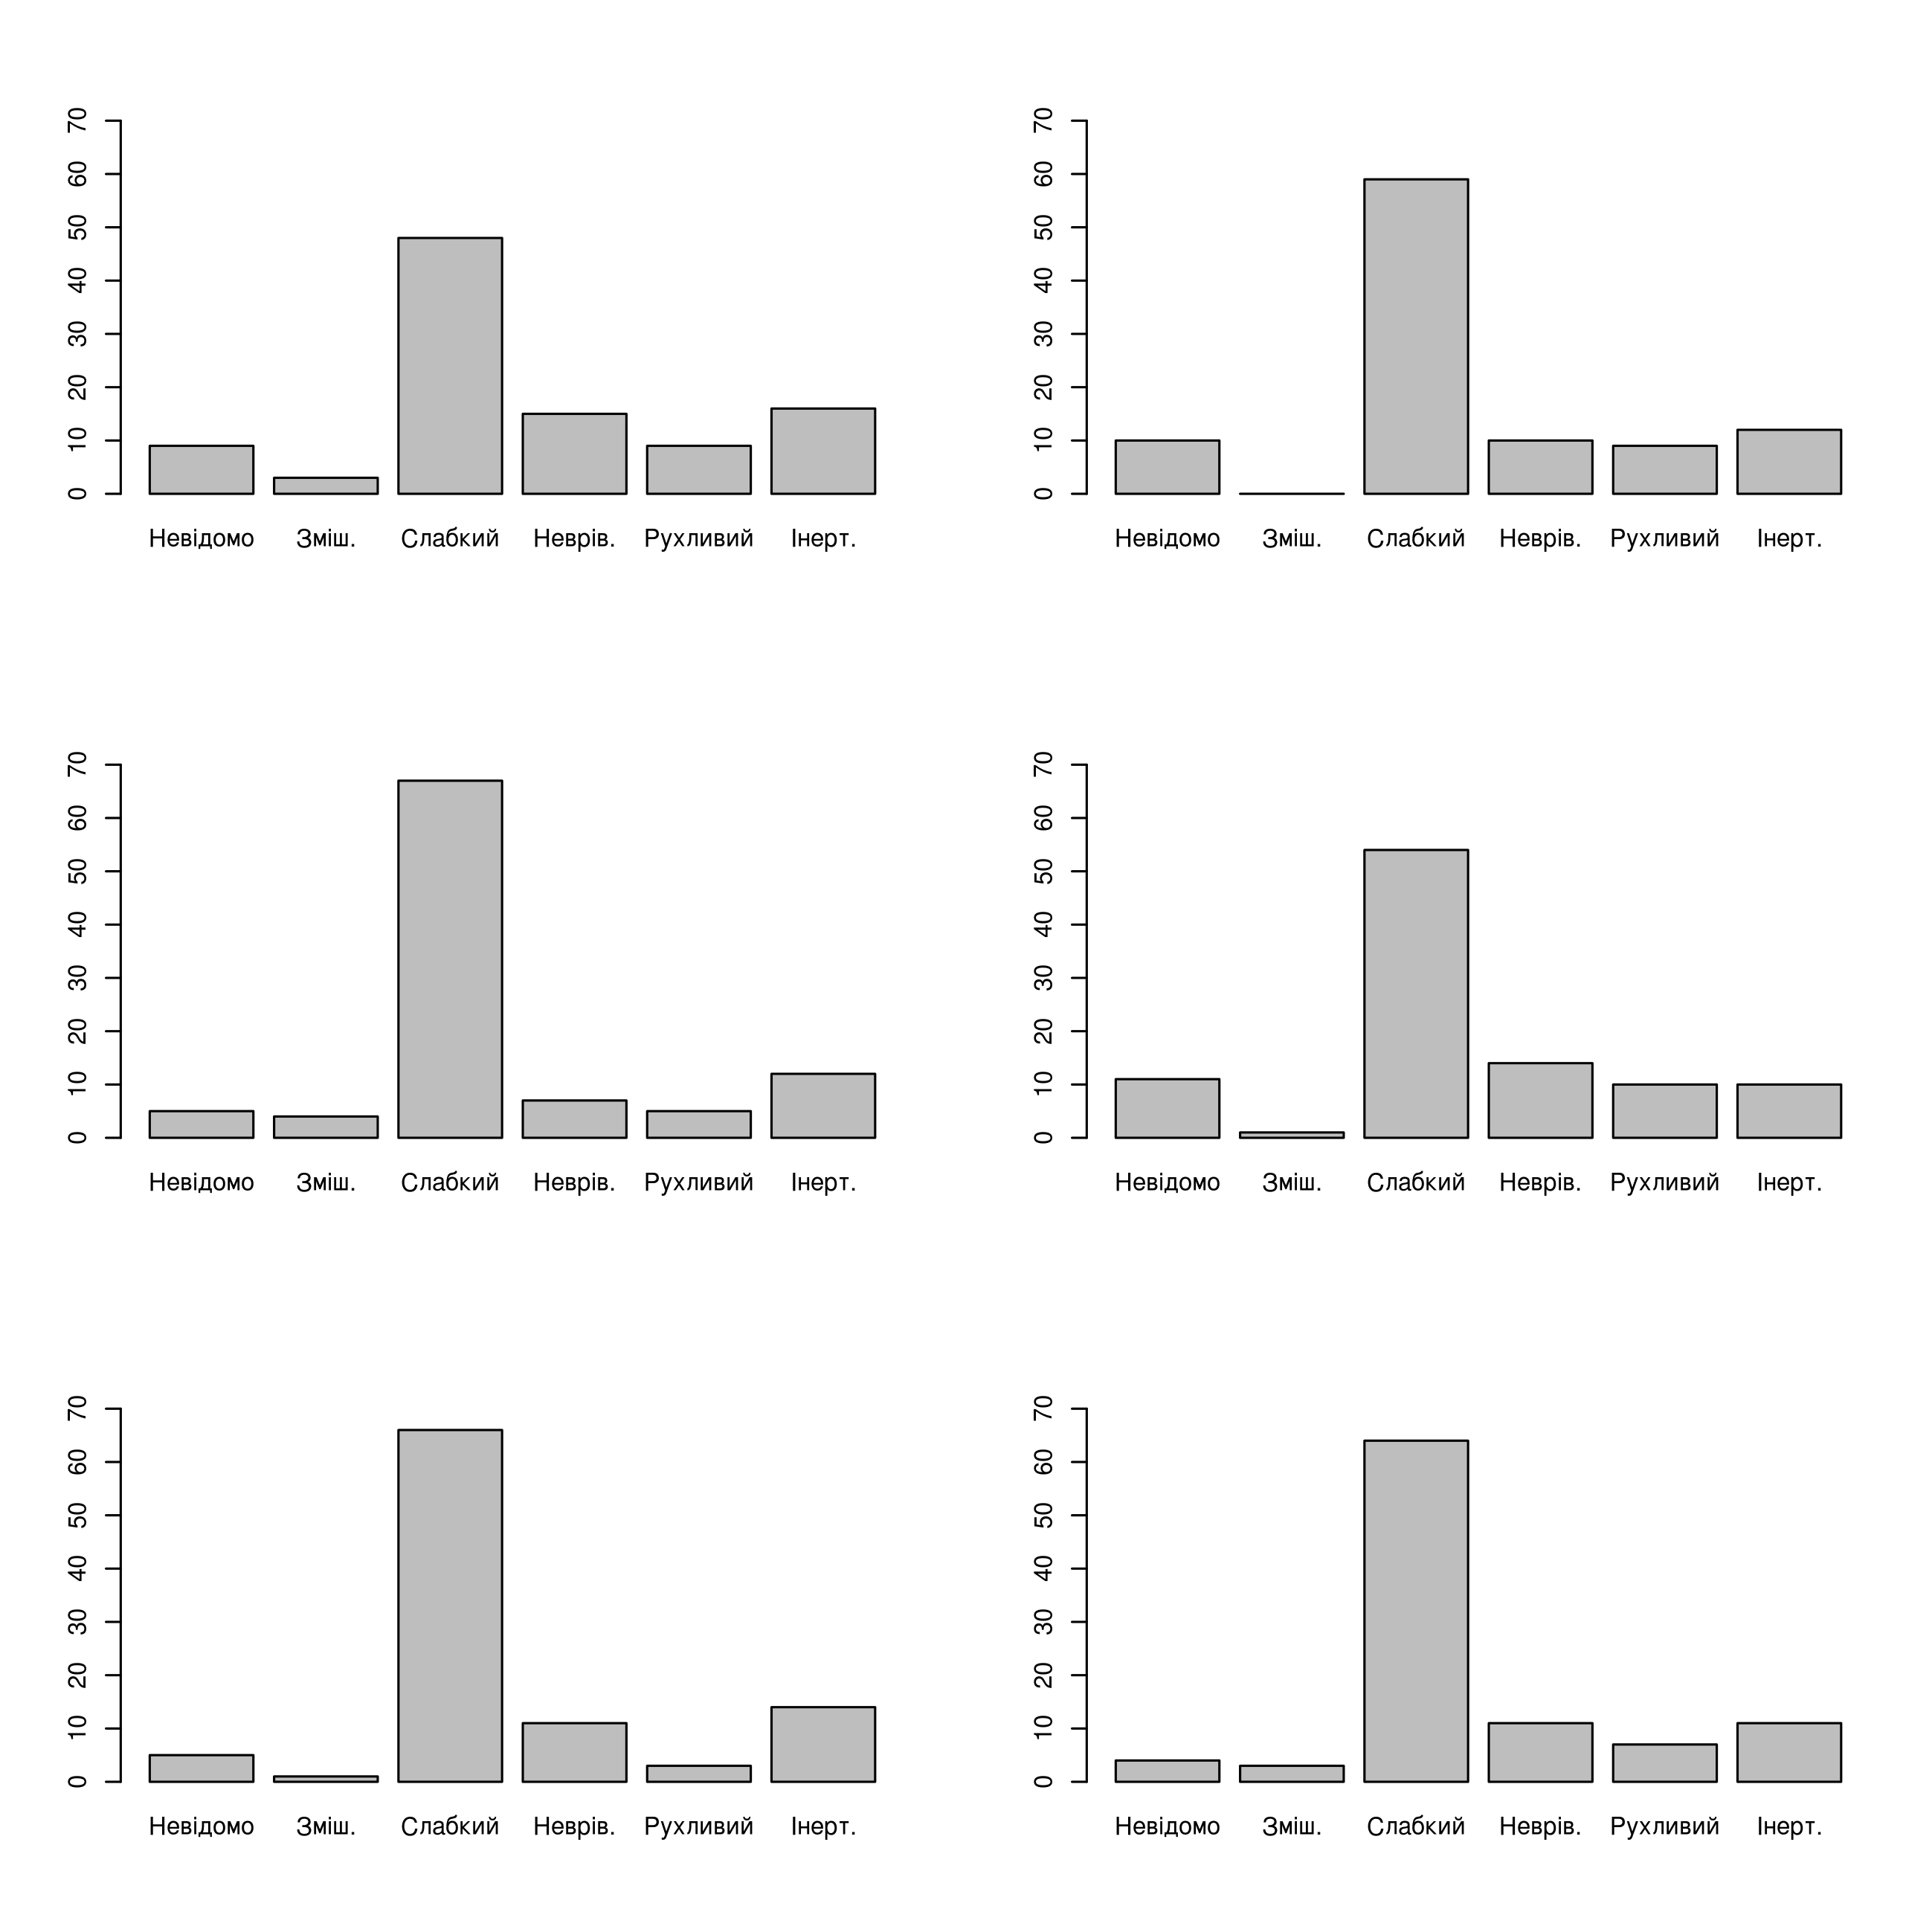
\includegraphics[width=\textwidth]{images/poisson_types}
%    \caption{Розбиття траєкторій по вибірках}
%    \label{fig:tapping:poisson:types}
%\end{figure}

\begin{figure}[h]
  \centering
  \begin{subfigure}[b]{0.45\textwidth}
    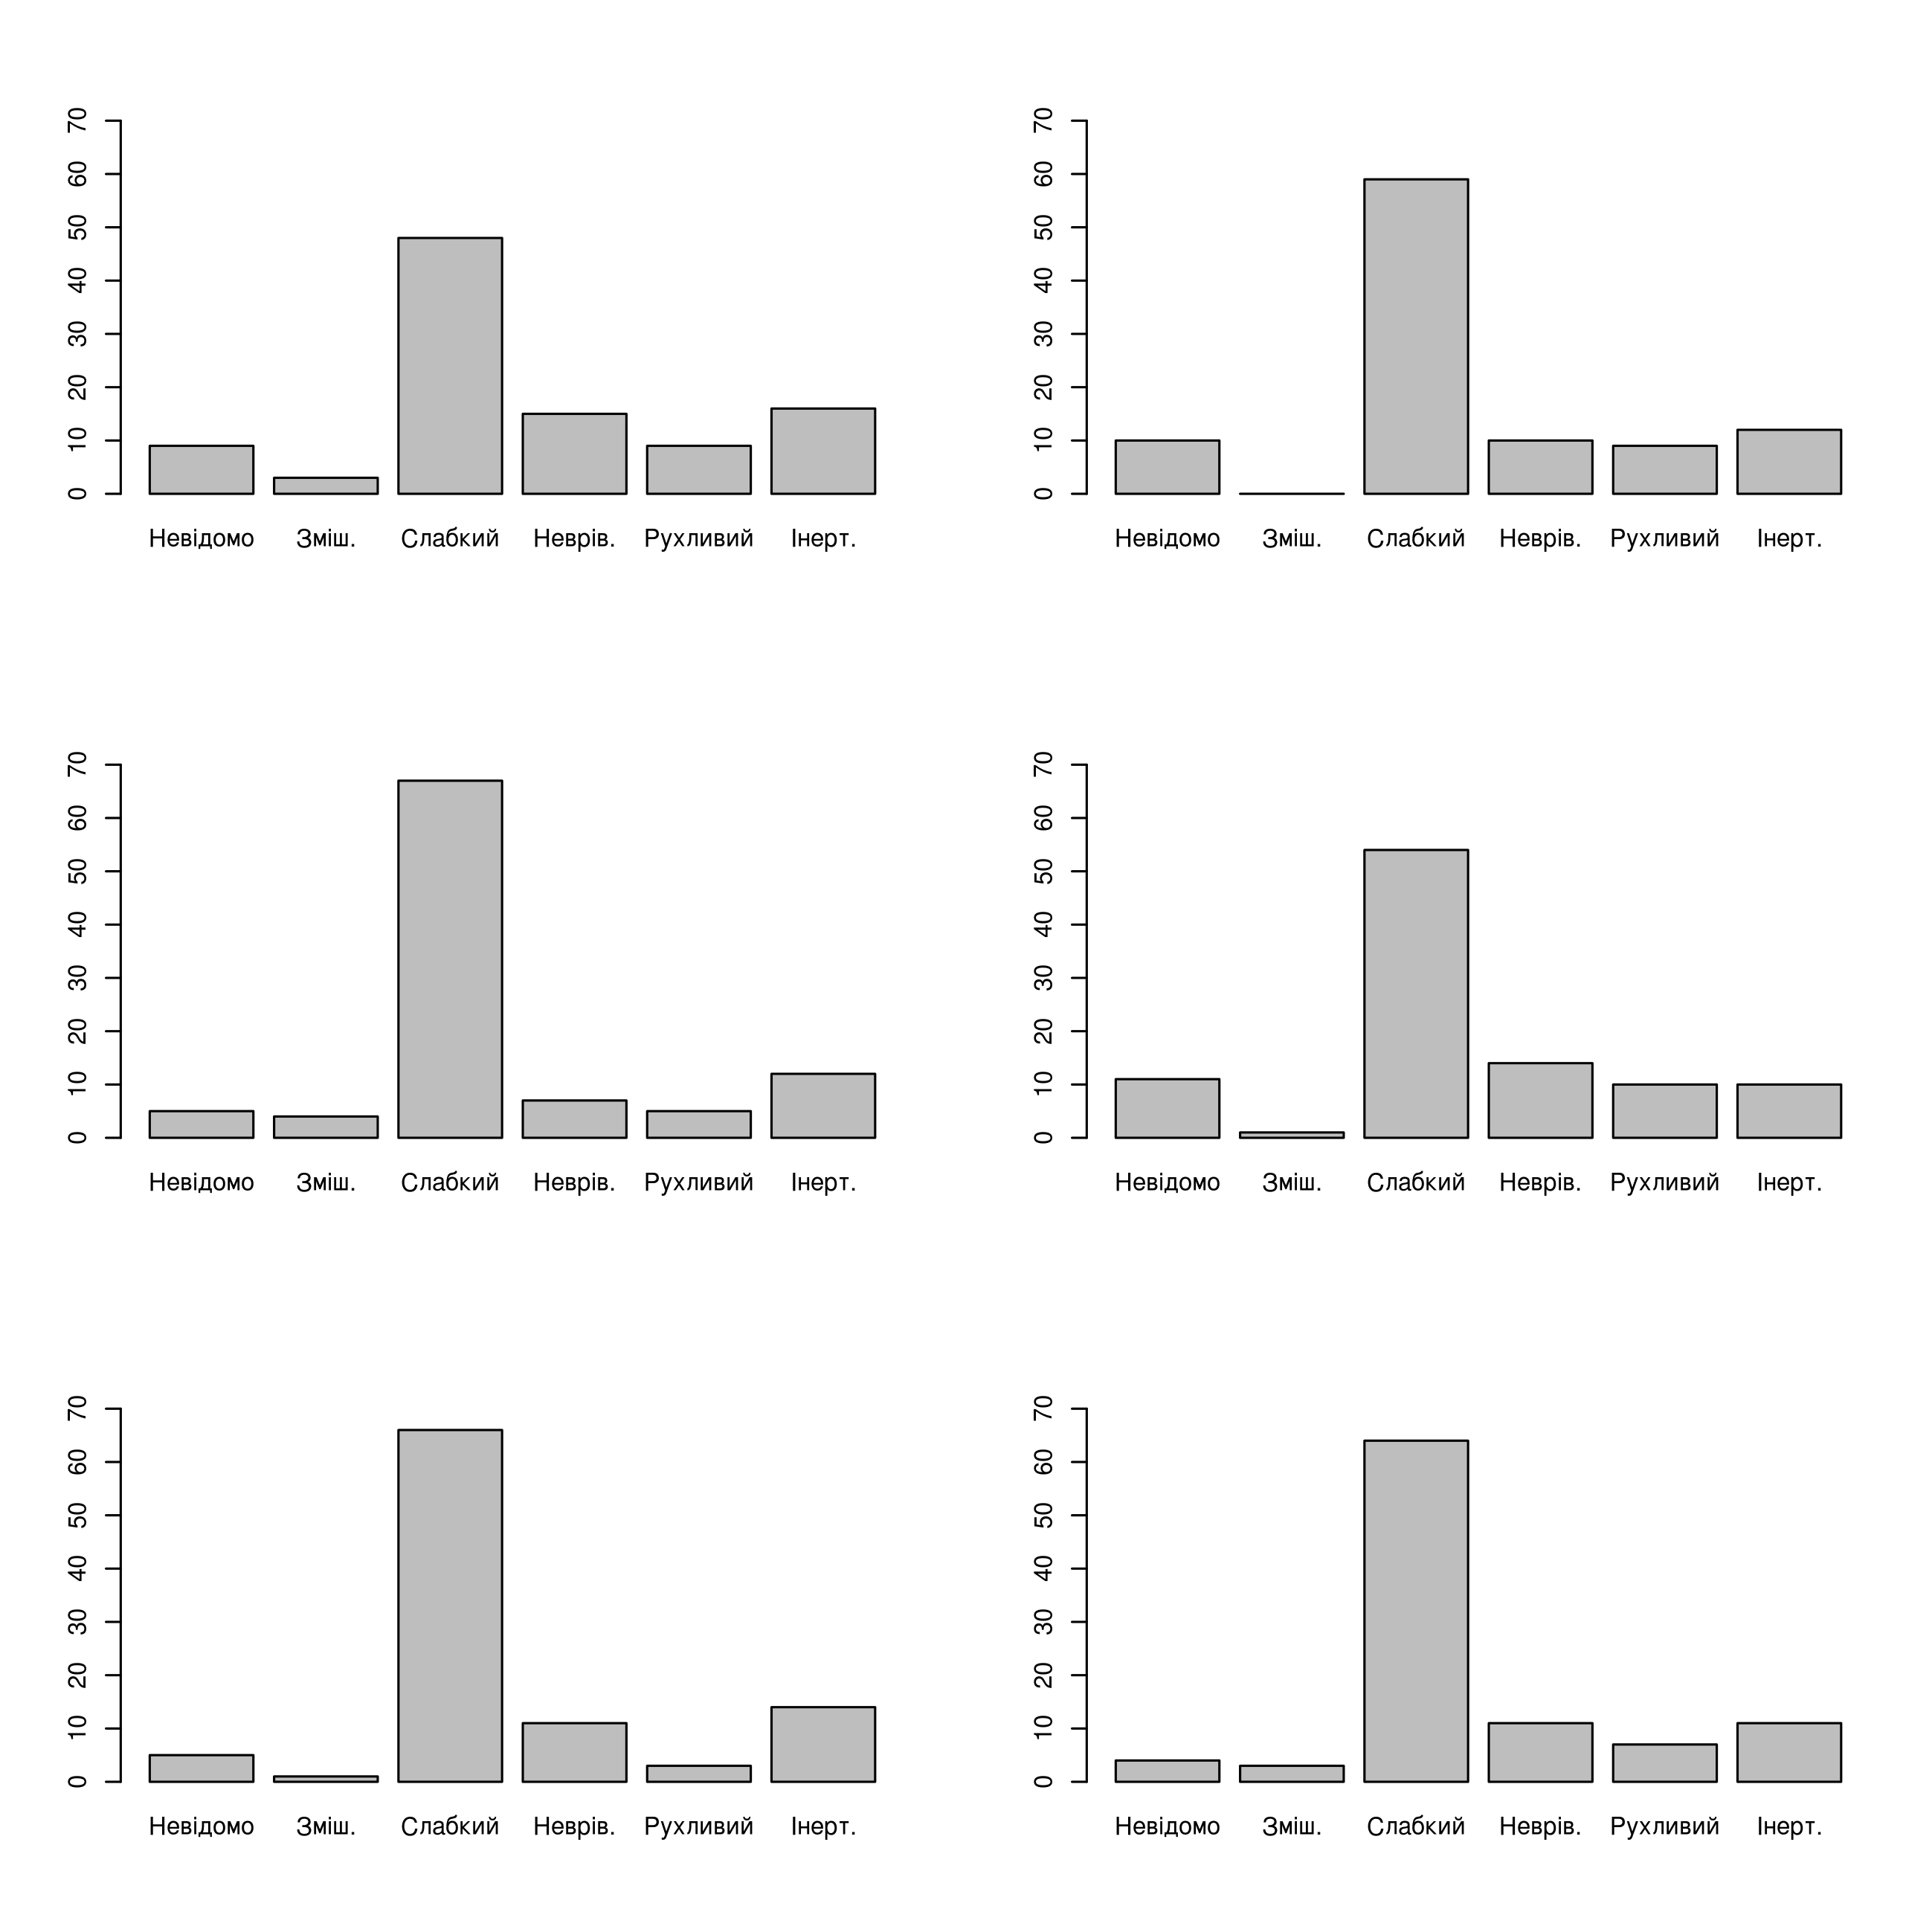
\includegraphics[width=\textwidth]{images/poisson_types}
    \caption{Звичайна школа}
    \label{fig:tapping:poisson:types}
  \end{subfigure}
  \begin{subfigure}[b]{0.45\textwidth}
    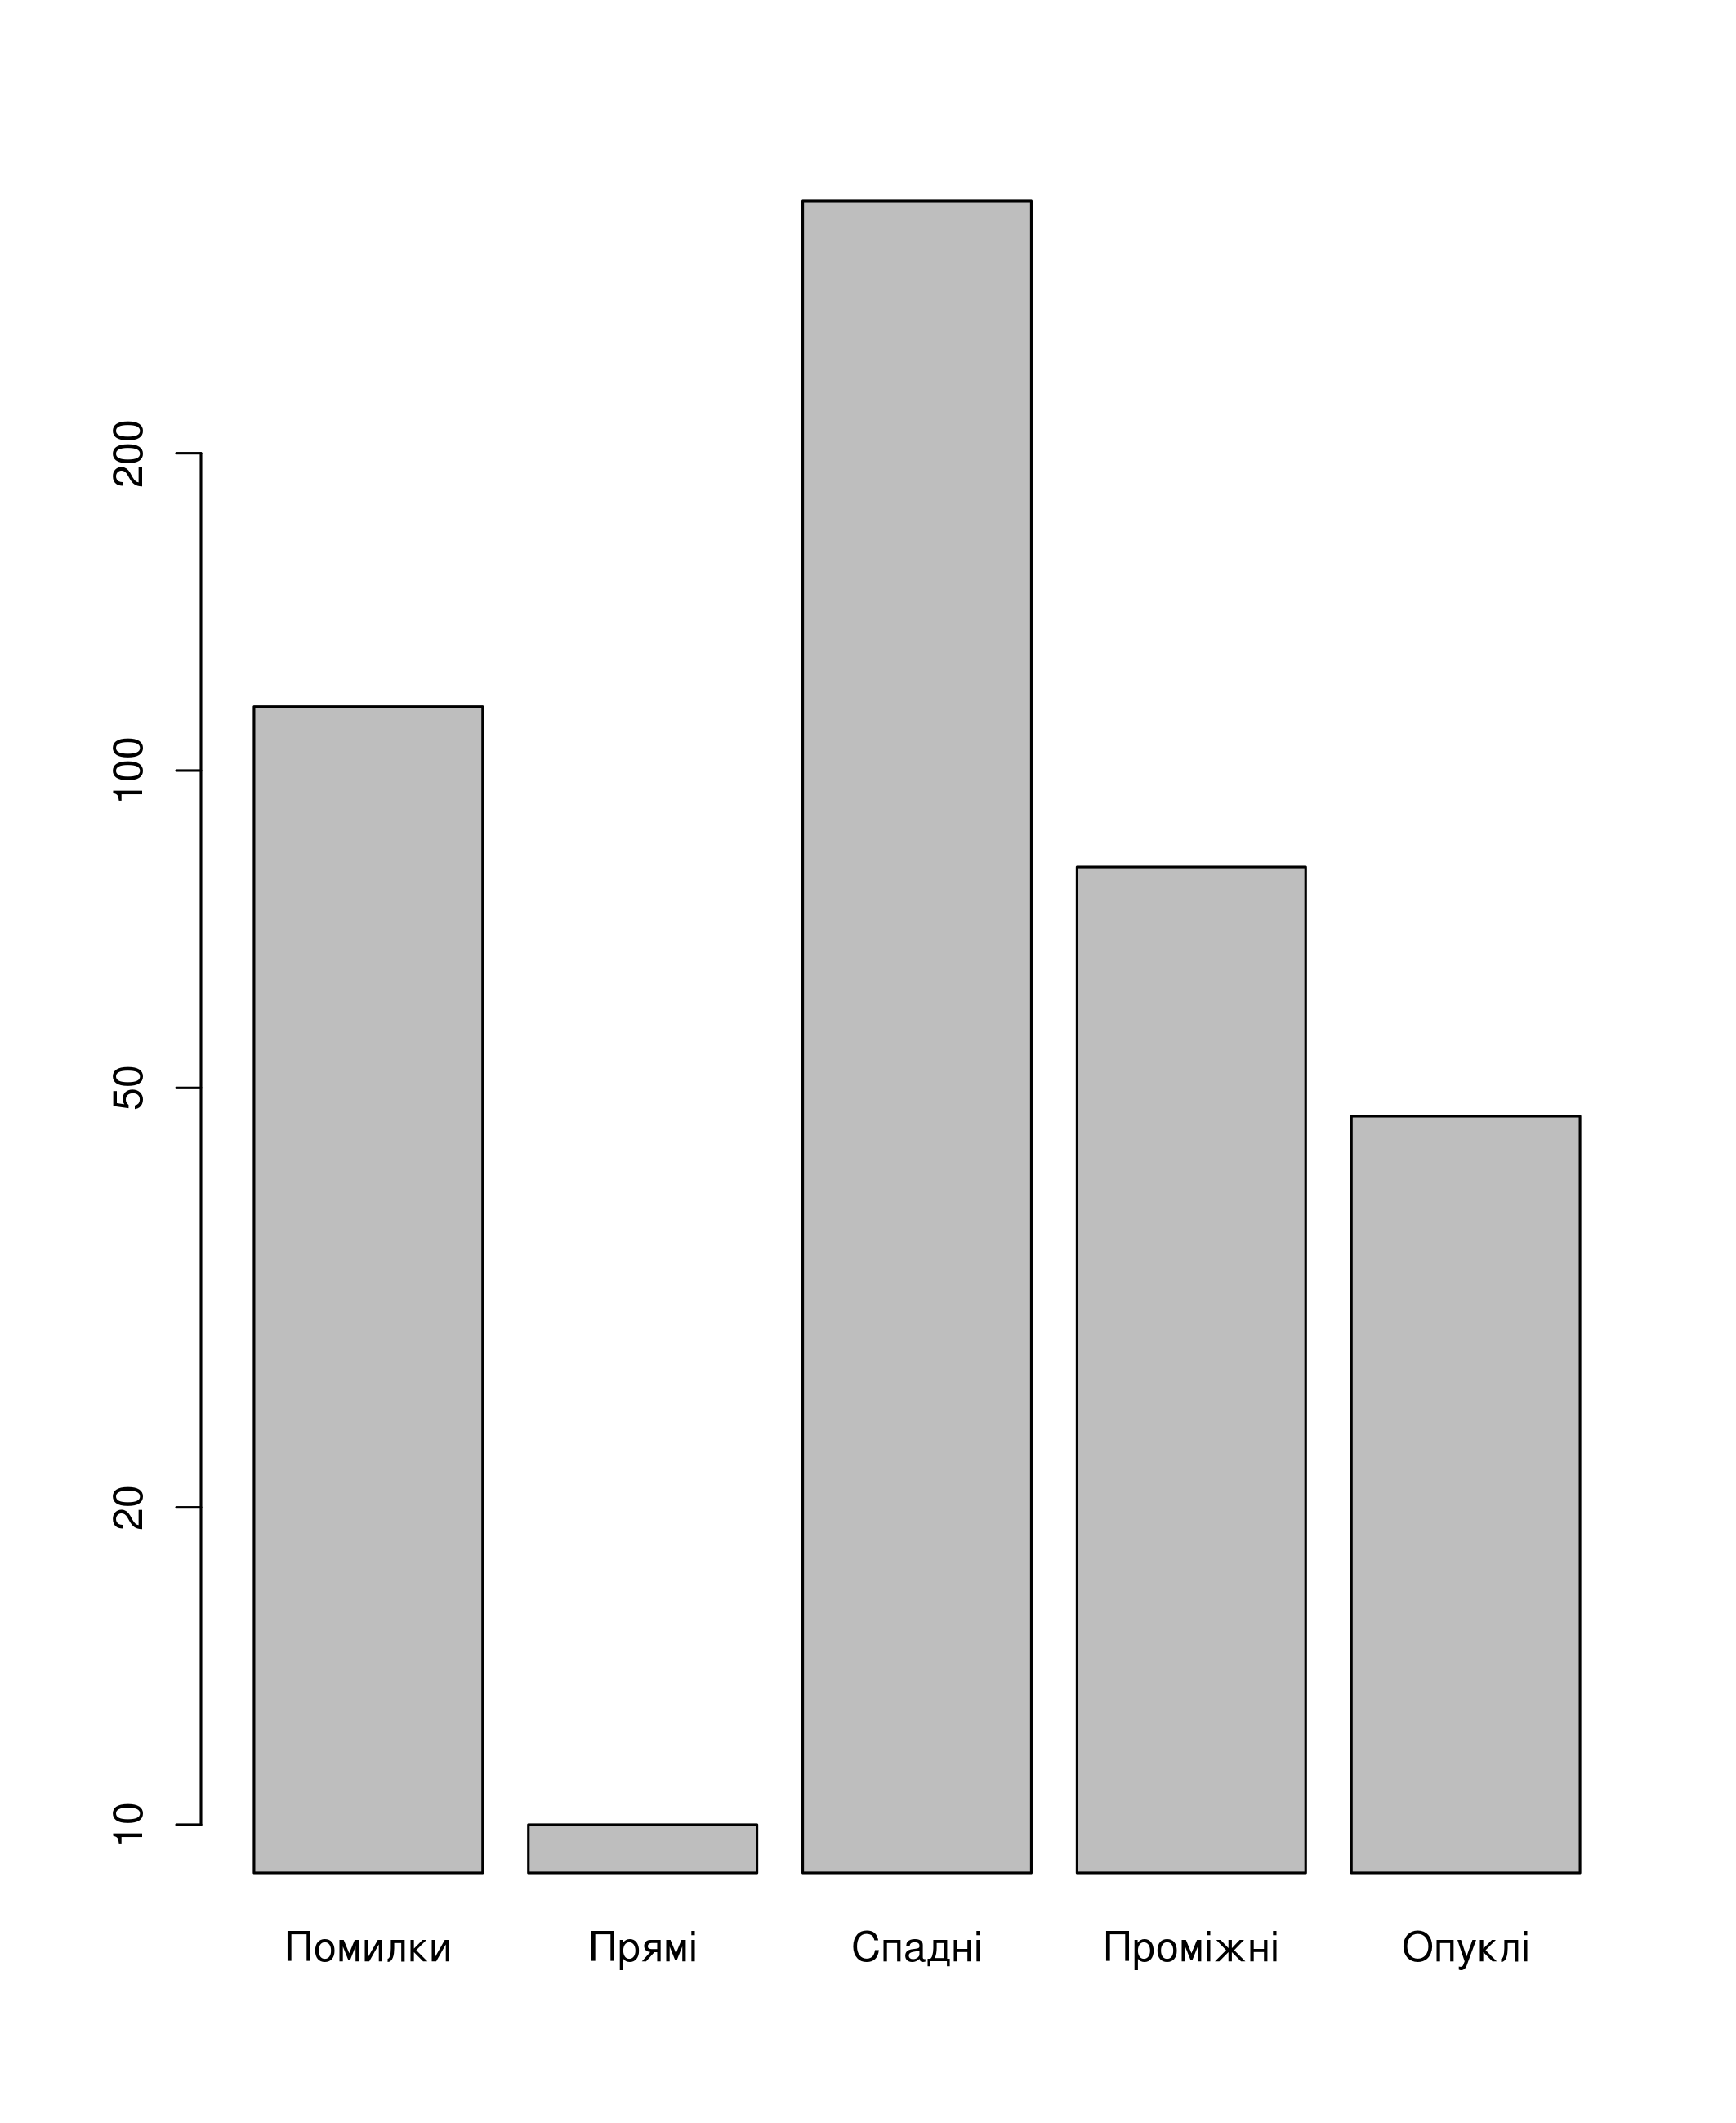
\includegraphics[width=\textwidth]{images/poisson_types_log}
    \caption{Логарифмічна шкала}
    \label{fig:tapping:poisson:types:log}
  \end{subfigure}
  \caption{Розбиття траєкторій по класах}
\end{figure}

\message{ !name(2_analysis.tex) !offset(-121) }
